\newcommand{\sheetnum}{%
	03
}
%\setcounter{section}{\sheetnum-3}
\newcommand{\tutorialtitle}{%
    Multilayer Perceptrons and the Backpropagation algorithm 
}
\newcommand{\tutorialtitleshort}{%
	MLPs and Backprop
}
% for slides
\subtitle{\sheetnum \tutorialtitle}

\maxdeadcycles=1000 % Workaround for ! Output loop---100 consecutive dead cycles because of too many figures

% The following use of algroithms does not work well with the notes:
%
%
%
%
% instead use the following for your algorithms:
%
%\begin{figure}[!t]
%\removelatexerror
%\begin{algorithm}[H]
    % your algo here
    %\label{alg:algolabel}
    %\caption{algocaption}
%\end{algorithm}
%\end{figure}
%\begin{algorithm}
% Below is the definition for the command \removelatexerror:
\makeatletter
\newcommand{\removelatexerror}{\let\@latex@error\@gobble}
\makeatother

\begin{document} %%%%%%%%%%%%%%%%%%%%%%%%%%%%%%%%%%%%%%%%%%%%%%%%%%%%%%%

\sheet{\sheetnum}{\tutorialtitleshort}

\ttopic{\tutorialtitle}

\columnratio{0.2,0.8}\textbf{}
\begin{paracol}{2}
%\setlength{\columnseprule}{0.1pt}
%\setlength{\columnsep}{5em}

\begin{rightcolumn}

% notes version will ignore it
\begin{frame}
\titlepage
\end{frame}

\begin{frame}
\tableofcontents
\end{frame}

\mode<all>
\section{MLPs are universal function approximators}

\begin{frame}\frametitle{\subsecname}

MLPs are universal function approximators. This means that, provided some assumptions are satisfied, they are capable of finding a function with which to map observations $\vec x$ to a their corresponding label $y_T$.

Moving forward we will focus only on \emph{scalar} values for the label $y_T$.

   \begin{block}{The universal approximation theorem by Funahashi (1989)\footnote
	{ Funahashi (1989) On the approximate realization of 
		continuous mappings by neural networks. Neur Netw, 2:183--192\\
		Hornik et al. (1989) Multilayer Feedforward Networks 
		are Universal Approximators. Neur. Netw, 2:359--366. }}
	\small
    	Let $y_T{(\vec{x})}$ be a continuous, real valued function 
    	over a compact interval $K$ and     
		\begin{equation} 
		{y}{(\vec{x}; \vec w)} = \sum_{i=1}^M \mathrm{w}_i^{21} 
		f\Big( \sum\limits_{j=1}^N \mathrm{w}_{ij}^{10} 
		  \mathrm{x}_j - \theta_i \Big)
		 \end{equation}
    	be a three-layered MLP with a non-constant, bounded, 
    	monotonously increasing and continuous function 
    	$f: \mathbb{R} \rightarrow \mathbb{R}$.\\
		\vspace{4mm}
	   \pause

		Then there exists a set of parameters 
		$M, N \in \mathbb{N}$ and $\mathrm{w}_i^{21}, 
		\mathrm{w}_{ij}^{10}, \theta_i \in \mathbb{R}$ 
		such that for every $\varepsilon > 0$:
		\begin{equation}
		\max_{\vec{x} \in K} \Big| \, y_T{(\vec{x})} - {y}{(\vec{x}; \vec w)} \,\Big| 
		\leq \varepsilon
		 \end{equation}
  \end{block}
  
\end{frame}


\mode*

\newpage

\mode<all>
\section{Ingredients for function fitting}

\begin{frame}\frametitle{\secname}

\mode<article>{
Fitting an MLP to a desired function $y_T(\vec x)$ requires the following:
}

\begin{enumerate}
\item 
\mode<article>{A cost function  with the objective to optimize it, often a minimization problem: $e(y_T, \vec x) \eqexcl \min$}
\mode<presentation>{A cost function:$e(y_T, \vec x) \eqexcl \min$}
\item A performance measure, a criterion for \emph{model selection}.
\mode<article>{Specifically, \\

the generalization \textbf{error} $E^G$ which is defined as:}	
\begin{equation} 
			E^G \quad := \quad \left<\,e\,\right>_{y_T, \vec{x}} 
			\quad = \quad \iint d \vec{x} \, dy_T \; 
				P_{(y_T, \vec{x})} \, e_{(y_T, \vec{x})}
\end{equation}

Because $P_{(y_T, \vec{x})}$ is not known, \mode<article>{we turn to the principle of empirical risk minimization (ERM).
According to ERM we can} approxomate $E^G$ by computing the empirilcal average $E^T$ using the available training data 
$\left\{\left(\vec x^{(\alpha)}, y_T^{(\alpha)}\right)\right\}, \alpha=1,\ldots,p$.
\mode<article>{The training error $E^T$ becomes:}

\begin{equation}
\text{batch training error:}\quad E^T=\sum_{\alpha=1}^{p} e^{(\alpha)}
\end{equation}
\mode<article>{
where $e^{(\alpha)}$ is the cost computed from a single observation $y(x^{(\alpha)};\vec w)$ and its corresponding label ($y_T^{(\alpha)}$). The superscript $^{(\alpha)}$ is used as an index of a specific point in the dataset.
}
\item A model with tunable parameters $\vec w$: MLP, connectionist neuron, \ldots
\item A learning algorithm\mode<article>{ for finding the set of parameters in our model that will minimize the cost function.\\
This can be done analytically (depending on some conditions) or through an iterative learning algorithm (e.g. gradient-based learning)}
\end{enumerate}

\end{frame}


\mode*

\newpage

\mode<all>
\subsection{Cost functions}
\begin{frame}\frametitle{\subsecname}
\mode<article>{
A cost function $e\tyxw$, quantifies the discrepancy between the model's prediction $y(\vec x; \vec w)$ and the label $y_T$ which $\vec x$ is assigned to.
}
Choosing a cost function accounts for 
\begin{enumerate}
\item the type of problem (i.e. regression vs. classification), 
\item how the model is penalized for different types of mistakes it can make such as:
small errors are tolerable, large errors are penalized less, etc.
\end{enumerate}
\mode<article>{
The choice of cost function has a direct effect on how the model learns. For example, we will later see in gradient-based learning how the error function can modulate how fast or slow a model learns.
}
\end{frame}

\subsubsection{Cost functions for Regression}

\begin{frame}\frametitle{\subsecname}

  \begin{tabular}{c c c}
    \parbox{4cm}{
      \[ \underbrace{\vec{x}
          \in \mathbb{R}^N
      }_{\text{feature vector}}
      \longrightarrow 
      \underbrace{y
      \in \mathbb{R}
      }_{\substack{\text{scalar}\\ \text{attribute}}}
      \]}
    & & 
    \parbox{8cm}{\footnotesize
      \begin{tabular}{l l}
	$y_T(\vec x)$: & true value of attribute \\
	$y(\vec{x}; \vec w)$: & predicted value of attribute \\
					& (e.g. by MLP)
      \end{tabular}
    }
  \end{tabular}
     \pause

  \begin{block}{individual cost $e\tyxw$}
    \begin{center} 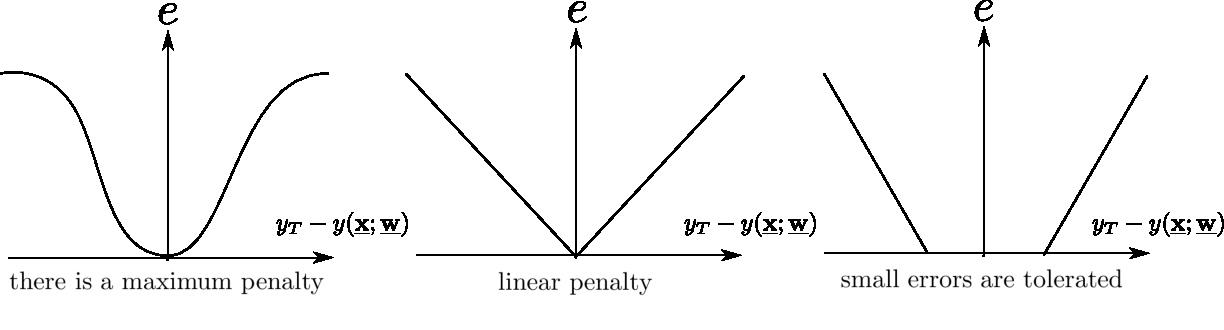
\includegraphics[width=12cm]{img/section1_fig17_v2.pdf} \end{center}
  \end{block}
\end{frame}

\begin{frame}\frametitle{Quadratic vs. linear error}

\begin{figure}[ht]
     \centering
     \savebox{\imagebox}{
	 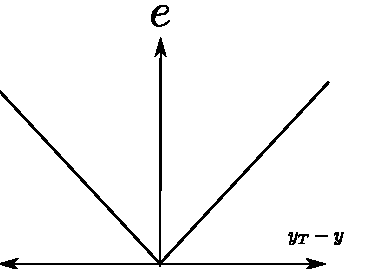
\includegraphics[width=0.4\textwidth]{img/section1_fig17_linear}}%
     \begin{subfigure}[t]{0.45\textwidth}
         \centering
         \usebox{\imagebox}% Place largest image
         \caption{linear error}
         \label{fig:quadratic}
     \end{subfigure}
     \hfill
     \begin{subfigure}[t]{0.45\textwidth}
         \centering
         \raisebox{\dimexpr.5\ht\imagebox-.5\height}{% Raise smaller image into place
         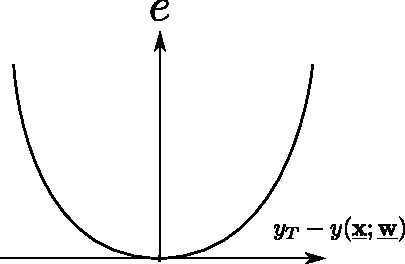
\includegraphics[width=0.99\textwidth]{img/section1_fig17_quadratic}
         }
         \caption{qudratic error}
         \label{fig:linear}
     \end{subfigure}
     \mode<article>{
     \caption{quadratic vs. linear error}
     }
	 \label{fig:quadratic_vs_linear}
\end{figure}


\begin{equation}
e_{\text{quadratic}}\tyxw := \frac{1}{2} \Big( y_{T}(\vec x) - y(\vec x;\vec w)\Big)^{2}
\label{eq:quadratic_error}
\end{equation}

\begin{equation}
e_{\text{linear}}\tyxw := \Big| y_{T}(\vec x) - y(\vec x;\vec w)\Big|
\label{eq:linear_error}
\end{equation}
\mode<article>{
The purpose of having $\frac{1}{2}$ in \eqref{eq:quadratic_error} is for convenience for when we calculate the derivative later. 
Both the quadratic and linear cost functions are symmetric. They therefore yield the same error regardless of the sign. However, the differences between them are:
}
\end{frame}
\begin{frame}\frametitle{Quadratic vs. linear error}
\begin{table}[h]
\centering
\caption{Differences between quadratic and linear cost}
\begin{tabular}{|c|c|}
\hline
quadratic                                                                                                    & linear                                                                                                  \\ \hline \hline
\begin{tabular}[c]{@{}c@{}}larger error $\leadsto$ larger penalty\\  (sensitive to outliers)\end{tabular} & \begin{tabular}[c]{@{}c@{}}constant increase in error\\  (more stable, robust to outliers)\end{tabular} \\ \hline
\begin{tabular}[c]{@{}c@{}}converges faster\\ but slow convergence\\ for small errors\end{tabular}           & constant convergence rate                                                                               \\ \hline
differentiable everywhere                                                                                    & \begin{tabular}[c]{@{}c@{}}not differentiable at zero\\ (not a huge problem)\end{tabular}               \\ \hline
\begin{tabular}[c]{@{}c@{}}max. likelihood of\\ Gaussian variable\end{tabular}                               &                                                                                                         \\ \hline
\end{tabular}
\end{table}

\end{frame}

\newpage

\begin{frame}\frametitle{Relation between quadratic error and Gaussian labels}

\mode<article>{
\paragraph{Relation between quadratic error and Gaussian labels}\\

}

Assume labels $y_T$ are conditionally Gaussian:

\begin{equation}
P(y_T|\vec x) = \mathcal{N}(y_T|\underbrace{y(\vec x;\vec w)}_{= \mu},\sigma^2)
\label{eq:gaussian_labels}
\end{equation}

\mode<article>{
Using the quadratic cost leads to a solution that corresponds to the same solution found from maximizing the (log-)likelihood\footnote{often, the log-likelihood is maximized for computational efficiency as the log replaces the product with a sum.} of the Gaussian labels:
}
\only<1>{
%\begin{figure}[h]
     %\centering
	%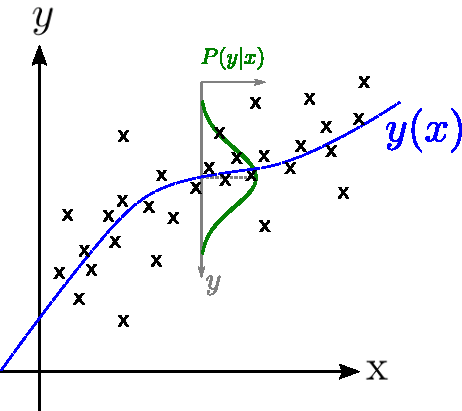
\includegraphics[width=0.4\textwidth]{img/gaussian_labels}
	%\caption{Gaussian distributed labels}
	%\label{fig:gaussian_labels}
%\end{figure}

\begin{figure}[ht]
     \centering
     \savebox{\imagebox}{
	 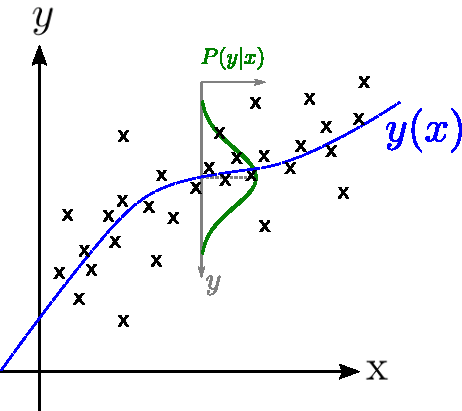
\includegraphics[width=0.37\textwidth]{img/gaussian_labels}}%
     \begin{subfigure}[t]{0.37\textwidth}
         \centering
         \usebox{\imagebox}% Place largest image
         \caption{guassian labels}
         \label{fig:quadratic}
     \end{subfigure}
     \hspace{2mm}
     \begin{subfigure}[t]{0.37\textwidth}
         \centering
         \raisebox{\dimexpr.5\ht\imagebox-.5\height}{% Raise smaller image into place
         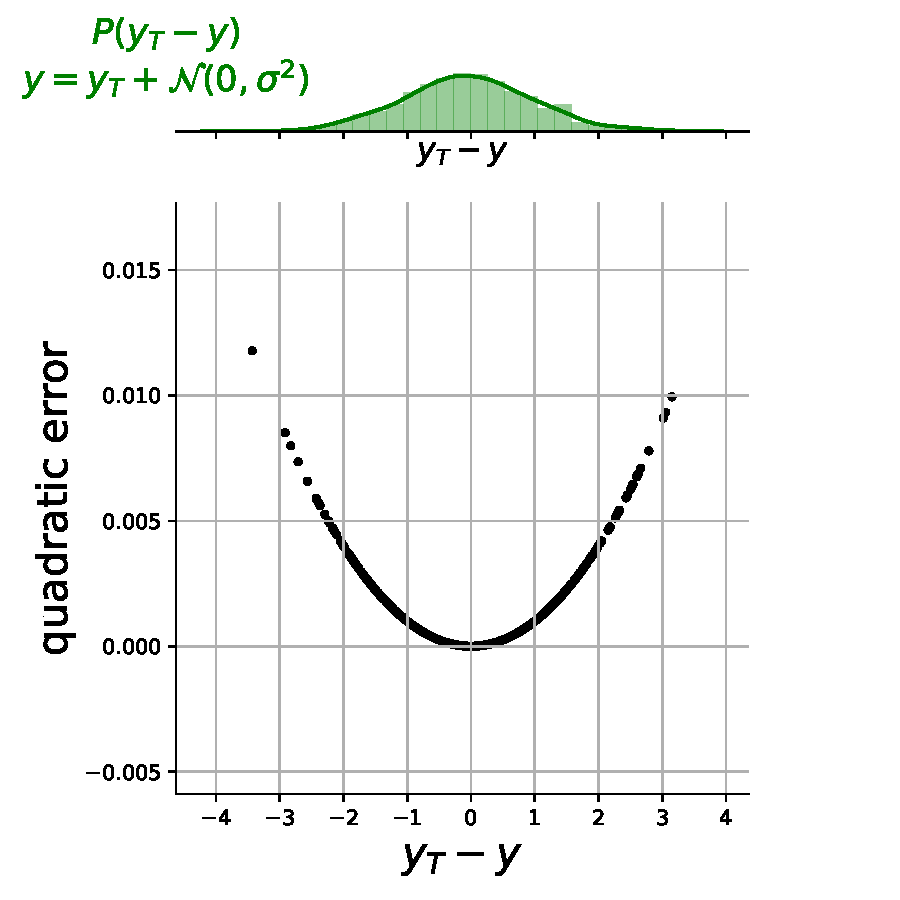
\includegraphics[width=0.99\textwidth]{img/qudaratic_conditional}
         }
         \caption{aggregate density}
         \label{fig:linear}
     \end{subfigure}
     \mode<article>{
     \caption{quadratic error and guassian labels}
     }
	 \label{fig:quadratic_density_gaussian}
\end{figure}
}
\only<2>{
\begin{align}
\vec w^* \in \argmin_{\vec w} \ETw 
\iff& 
\argmax_{\vec w} \underbrace{\prod_{\alpha=1}^{p} \mathcal{N}(y_T|{y(\vec x;\vec w)},\sigma^2)
}_{
\text{likelihood function } \mathcal{L(\vec w)}
}\\
&=
\argmin_{\vec w}
\underbrace{
 \lbrack - \ln \mathcal{L(\vec w)}\rbrack
 }_{\text{neg. log likelihood}}
\end{align} 
}


\end{frame}

\mode<article>{
This property makes the quadratic cost function the standard choice for regression.
}

\subsubsection{Cost functions for binary classification}

\begin{frame}\frametitle{\subsubsecname\\Deriving the cross entropy cost function for binary classification}

\mode<article>{
\paragraph{Deriving the cross entropy cost function for binary classification}\\
}

\begin{itemize}
\item[]\underline{Data}:\\

\begin{equation}
\Big\{ \left( \vec x^{(\alpha)}, y_T^{(\alpha)} \right) \Big \}_{\alpha=1}^{p}
\end{equation}

with 
$$
\vec x^{(\alpha)} \in \R^N\;\;,\;\; y_T^{(\alpha)} \in \{{\color{red}0}, {\color{blue}1}\}.
$$

generated by
\begin{equation}
\left( \vec x^{(\alpha)}, y_T^{(\alpha)} \right) \stackrel{\iid}{\sim} P_{\text{data}}(\vec x, y)
\end{equation}

\pause

\item[]\underline{Model}:\\

MLP, scalar output \mode<article>{interpreted as probability that $y(\vec x; \vec w)=1$. In other words the probability of $\vec x$ belonging to class '1' (the positive class):}

\begin{equation}
y(\vec x;\vec w) =: P_{\text{model}} ({\color{blue}y=1}|\vec x;\vec w) \;\; \text{and} \;\; P_{\text{model}} ({\color{red}y=0}|\vec x; \vec w) = 1-y(\vec x;\vec w)
\end{equation}

for the \textcolor{blue}``positive'' and ``negative''/``other'' class respectively.

\end{itemize}

\end{frame}

\begin{frame}\frametitle{Cost function derivation via minimization of \\the Kullback-Leibler divergence}

\mode<article>{
\paragraph{The Kullback-Leibler divergence }\\

}

$\dkl(P||Q)$ is a measure of how much a probability distribution $P$ differs from another distribution $Q$.

Properties of the KL-divergence:

\begin{itemize}
\item $\dkl = 0$ iff. both distribution are \emph{identical}.
\item Otherwise $\dkl > 0$.
\item Does not qualify as a metric because it is not symmetric. For different distributions P and Q: $\dkl(P_||Q) \ne \dkl(Q||P)$
\end{itemize}

\end{frame}

\begin{frame}\frametitle{Cost function derivation via minimization of the Kullback-Leibler divergence}
 
From KL-divergence to binary cross entropy loss:
\only<1>{

\begin{align}
\dkl\left(\, P_{\text{data}}(\vec x, ) \,||\, P_{\text{model}}(\vec x, y) \,\right)
= \iint d \vec x dy P_{\text{data}}(\vec x, y)
\ln 
\left( 
\frac{P_{\text{data}}(\vec x, y)}{P_{\text{model}}(\vec x, y)}
\right)
\end{align}

\mode<article>{
Integrating w.r.t. $y$ $\corresponds$ sum over the set of all possible values for $y$, which is $\{0,1\}$ in this case:
}
}
\definecolor{darkgreen}{rgb}{0,0.6,0}
\begin{align}
\only<1,2>{
\dkl&\left(\, P_{\text{data}}(\vec x, y) \,||\, P_{\text{model}}(\vec x, y) \,\right)\\
&= \int_{\R^N} d \vec x \sum_{y \in \{0,1\}} P_{\text{data}}(\vec x, y) \ln 
\left( 
\frac{P_{\text{data}}(\vec x, y)}{P_{\text{model}}(\vec x, y)}
\right)\\
}
\only<1,2>{
&= \int_{\R^N} d \vec x \sum_{y \in \{0,1\}} 
	\underbrace{
		P_{\text{data}}(\vec x)P_{\text{data}}(y | \vec x)
	}_{
		\substack{
		=P_{\text{data}}(\vec x, y)\\(\text{Bayes' rule})
		}
	}
	\ln 
	\left( 
		\frac{ P_{\text{data}}(\vec x)P_{\text{data}}(y | \vec x) }
		{
		\smash{
			\underbrace{
				P_{\hcancel[red]{\text{model}}}(\vec x)
				}_{
				\substack{
					\color{red}\text{discriminative model}\\
					\color{red}\text{not a generative model}\\
					\color{red}\text{replace with }
					{\color{cyan} P_{\text{data}}(\vec x)}
				}%substack
			}%underbrace
			\hspace{-5mm}
			P_{\text{model}}(y | \vec x)
		}%smash
		}%frac(lower)
	\right) \\
}
\only<2,3,4>{
&= \int_{\R^N} d \vec x \sum_{y \in \{0,1\}} 
	\underbrace{
		\color{darkgreen}
		P_{\text{data}}(\vec x)
	}_{\text{indep. of } y}
	P_{\text{data}}(y | \vec x)
	\ln 
	\left( 
	\frac{
		{ \color{cyan} P_{\text{data}}(\vec x) }
		{ \color{violet} P_{\text{data}}(y | \vec x) }
	}
	{
		{ \color{cyan} P_{\text{data}}(\vec x) }
		{ \color{brown} P_{\text{model}}(y | \vec x) }
	}%frac(lower)
	\right) \\
}
\only<3,4>{
&= \underbrace{
	\int_{\R^N} d \vec x \,
	{ \color{darkgreen} P_{\text{data}}(\vec x) }
	\sum_{y \in \{0,1\}}
	P_{\text{data}}(y | \vec x)
	\ln 
	\lbrack { \color{violet} P_{\text{data}}(y | \vec x) } \rbrack
	}_{\text{indep. of model parameters } \vec w} \\
	&\qquad- \int_{\R^N} d \vec x \,
		{ \color{darkgreen} P_{\text{data}}(\vec x) }
		\underbrace{
			\sum_{y \in \{0,1\}}
			P_{\text{data}}(y | \vec x)
			\ln
			\lbrack {\color{brown} P_{\text{model}}(y | \vec x) } \rbrack
		}_{
		\substack{
		\text{\textbf{cross entropy} between } \\
		\text{data \& model distributions given }\vec x}
		}
}
\end{align}

\mode<presentation>{
\only<4>{
Apply ERM on the \textbf{cross entropy} term.
}
}

\end{frame}

\begin{frame}\frametitle{ERM}

\mode<article>{
ERM for computing cross entropy loss using the training data:
}
\mode<presentation>{
\vspace{-5mm}
}

\begin{align}
\onslide<1->{
\ETw &= \frac{1}{p} \sum_{\alpha=1}^{p} - \bigg( \;
	\sum_{y\in\{{\color{red}0},{\color{blue}1}\}} P_{\text{data}}(y | \vec x^{(\alpha)})
	 \ln \lbrack P_{\text{model}}(y | \vec x^{(\alpha)}) \rbrack
	 \;\bigg)\\
	 &= \frac{1}{p} \sum_{\alpha=1}^{p} - \bigg( \;
	P_{\text{data}}({\color{blue}y=1} | \vec x^{(\alpha)})
	 \ln \lbrack P_{\text{model}}({\color{blue}y=1} | \vec x^{(\alpha)}) \rbrack \\
	 &\qquad\qquad\qquad+
	 P_{\text{data}}({\color{red}y=0} | \vec x^{(\alpha)})
	 \ln \lbrack P_{\text{model}}({\color{red}y=0} | \vec x^{(\alpha)}) \rbrack 
	  \;\bigg)\\
}
\onslide<2->{
	 &= \frac{1}{p} \sum_{\alpha=1}^{p} - \bigg( \;
		{\color{blue}y_T^{(\alpha)}} \cdot
	 \ln \lbrack {\color{blue}y(\vec x^{(\alpha)};\vec w)} \rbrack
	 + ( {\color{red}1-y_T^{(\alpha)}} ) \cdot
	 \ln \lbrack {\color{red}1-y(\vec x^{(\alpha)};\vec w)} \rbrack
	 \;\bigg)\\
}
\onslide<3->{
	 &= \frac{1}{p} \sum_{\alpha=1}^{p} \bigg( -
		{\color{blue}y_T^{(\alpha)}} \cdot
	 \ln \lbrack {\color{blue}y(\vec x^{(\alpha)};\vec w)} \rbrack
	 - ( {\color{red}1-y_T^{(\alpha)}} ) \cdot
	 \ln \lbrack {\color{red}1-y(\vec x^{(\alpha)};\vec w)} \rbrack  \;\bigg) \\
	 &= \frac{1}{p} \sum_{\alpha=1}^{p} e\tyxwalpha
}
\end{align}

Extendable to multi-class cross entropy alongside \emph{softmax} normalization.

\end{frame}

\mode*

\newpage

\mode<all>
\section{Gradient-based learning}

\begin{frame}\frametitle{Minimizing the training error}
	Training error $E^T$ for the training set $\left\{\vec x^{(\alpha)}, y^{(\alpha)}_{T}\right\}$: 
    \begin{equation}
        \ETw = \frac{1}{p} \sum\limits_{\alpha = 1}^p 
					e\tyxwalpha
    \end{equation}
    
    \mode<article>{
    The objective is to minimize the training error w.r.t. the model parameters $\vec w$. That is
    }
    
    \begin{equation}
        \ETw \eqexcl \min_{\vec w} \quad \Rightarrow \quad \vec w^{*} = \argmin_{\vec w} \ETw
    \end{equation}

    \begin{figure}[h]
        \centering
        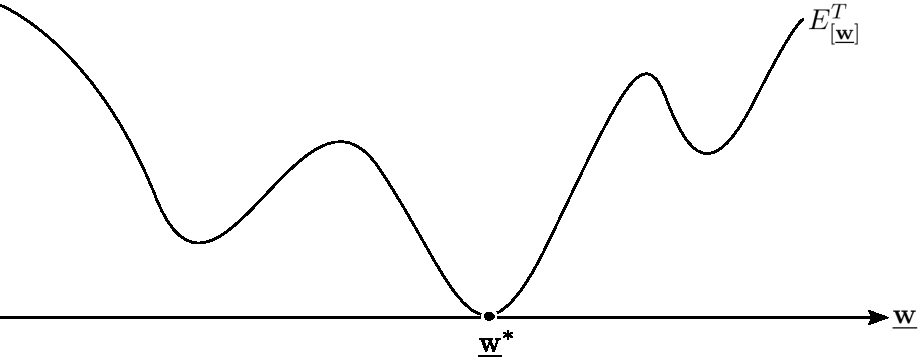
\includegraphics[height=3.25cm]{img/section1_fig19_no_steps}
        \caption{Training error with minimum at $\vec w^{*}$}
        \label{fig:training_error} 
    \end{figure}
    
    \pause 
    
    \question{What is the strategy for finding $\vec w^{*}$ analytically?}

\end{frame}

\subsection{Finding the minumum of the training error analytically}

\begin{frame}\frametitle{\subsecname}

    Example with a simple connectionist neuron model
    with parameters
    $$\vec w = (w_{0}, w_{1}, \ldots, w_{N})^{\top}$$\\


    - The strategy for finding the minimum of a function $\ETw$ analytically is as follows:
    \begin{enumerate}
    \item Compute the gradient w.r.t. $\vec w$ by taking the first partial derivatives w.r.t to each component in the vector $\vec w$
    \begin{equation}
        \frac{\partial \ETw}{\partial \vec w} = \left(\,
        \frac{\partial \ETw}{\partial w_{0}}, \,
        \frac{\partial \ETw}{\partial w_{1}}, \,\ldots\,,\, 
        \frac{\partial \ETw}{\partial w_{N}}\,
        \right)^{\top}
        \label{eq:gradient_partial}
    \end{equation}
    The gradient $\frac{\partial \ETw}{\partial \vec w}$ has the same dimensionality as $\vec w$.
    
    \item Set the gradient to zero: $\frac{\partial \ETw}{\partial \vec w} \eqexcl \vec 0$
    \item Solve for $\vec w$ to find extrema.
    \item Select solution corresponding to global minimum.
    
    \end{enumerate}
    
    \mode<presentation>{
    Caveat: Not always applicable. Closed-form solution infeasible for complex models such as MLPs.
    Instead: Iterative learning algorithm gradient descent.
    }
\end{frame}

\subsection{Gradient descent}

\begin{frame}\frametitle{Finding the minumum of $\ETw$ iteratively}

\mode<article>{

Learning from gradient descent is an alternate approach for finding the minimum of a function, when the closed-form solution is not available.

}
    \begin{figure}[h]
        \centering
        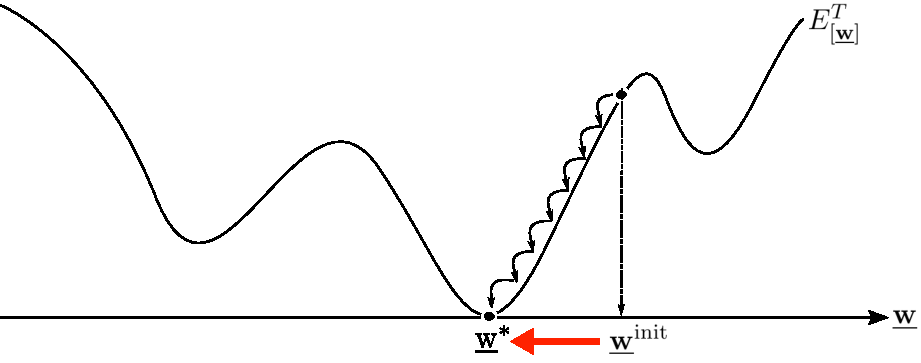
\includegraphics[height=3.25cm]{img/section1_fig19}
        \caption{Minimzing the training error iteratively via gradient descent}
        \label{fig:minimize_via_gradient_descent} 
    \end{figure}
    
    \only<1>{
    For our connectionist neuron example:
    \begin{equation}
    		w_{j}(t+1) \quad=\quad w_{j}(t) 
				\;\;{\color{red}-}\;\;
				\underbrace{{\eta}}_{ 
						\substack{\text{learning} \\ \text{step} } }
                        \cdot
				\underbrace{\frac{\partial \ETw}{
					\partial \mathrm{w}_{j}}}_{
						\substack{
							\text{\textcolor{red}{``gradient''}} 
			} }
            \label{eq:gradient_descent_neuron}
    \end{equation}
    
    with $j=0,\ldots,N$
    
    $\vec w^{\mathrm{init}}$ is bascially a random guess of where the solution might be and going against the gradient will potentially move us closer to the minimum. 
    }
	\only<2,3>{
    For an MLP:
    \begin{equation}
		w_{ij}^{v'v}(t+1) \quad=\quad w_{ij}^{v'v}(t) 
				\;\;{\color{red}-}\;\;
				\underbrace{\eta}_{ 
						\substack{\text{learning} \\ \text{step} } }
                        \cdot
				\underbrace{\frac{\partial \ETw}{
					\partial \mathrm{w}_{ij}^{v'v}}}_{
						\substack{
							\text{\textcolor{red}{gradient vector}} 
			} }
            \label{eq:gradient_descent_mlp}
    \end{equation}
    }
    
    \mode<article>{
    
    The learning step (learning rate) $\eta$ modulates the magnitude of our update. $\eta$ can be treated as a constant but we will also see how the value of $\eta$ can change over time, i.e. $\eta(t)$.
    }
    \only<3>{
    \question{Why do we \underline{subtract} the gradient from the current value of $w_{ij}^{v'v}(t)$?}
    }
    
    \mode<article>{
    
    The gradient describes the slope. Adding it will move us upwards and potentially maximize our function. Gradient-based learning with the intention of maximizing some function is referred to as hill climbing or gradient \emph{ascent}.
    }
    
    \only<4>{
    \question{So what's the downside of using gradient descent?}\\
    }
\end{frame}

\mode<article>{

    - The solution we find heavily depends on the initial position we started from. Indeed, gradient descent will reduce our cost each step but it does not guarantee that it will find the global minimum and will also stop at a local minimum. The slope in both cases is equal to zero.
    }

\begin{frame}\frametitle{\subsecname}
    
   \mode<presentation>{
    
    \textbf{So what's the downside of using gradient descent?}\\
    
    }
    
    \begin{figure}[h]
        \centering
        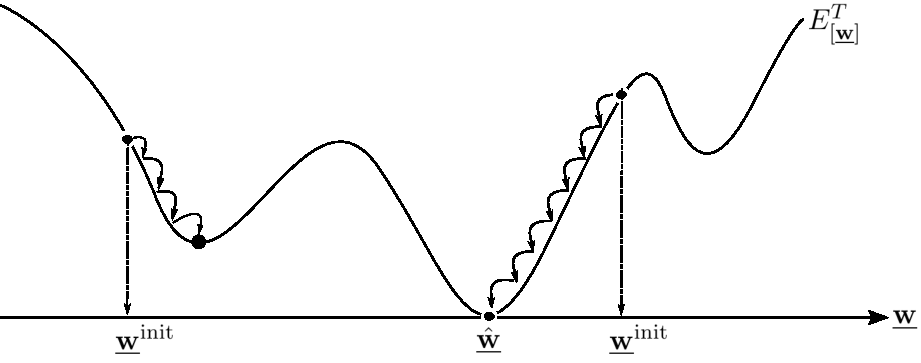
\includegraphics[height=3.25cm]{img/section1_fig19_local}
        \caption{Gradient descent finds local minima. We therefore denote the solution with $\hat{\vec w}$}
        \label{fig:minimize_via_gradient_descent_local} 
    \end{figure}
    
\end{frame}

\subsection{Gradient calculation: Connectionist neuron}

\begin{frame}\frametitle{Gradient calculation: Connectionist neuron}
    
    Recall the previous example with the connectionist neuron:
    
    \begin{figure}[h]
        \centering
        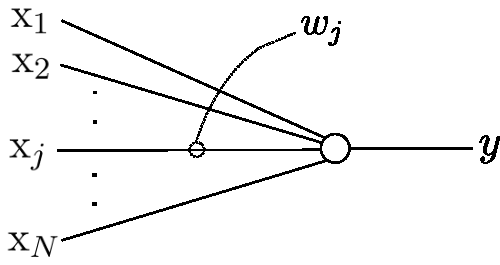
\includegraphics[height=2.5cm]{img/linearNeuron_y}
        \mode<article>{
        \caption{Connctionist neuron}
        }
        \label{fig:neuron} 
    \end{figure}
    
    Gradient descent updates the weights using:
    \begin{equation}
    		w_{j}(t+1) \quad=\quad w_{j}(t) 
				\;\;{\color{red}-}\;\;
				\underbrace{{\eta}}_{ 
						\substack{\text{learning} \\ \text{step} } }
                        \cdot
				\underbrace{\frac{\partial \ETw}{
					\partial \mathrm{w}_{j}}}_{
						\substack{
							\text{\textcolor{red}{``gradient''}} 
			} }
    \end{equation}
    
\end{frame}
\begin{frame}
    
    \only<1>{
    Knowing that
    \begin{align}
		\frac{\partial \ETw}
			{\partial \mathrm{w}_{j}}
		\;&=\; \frac{1}{p} \sum_{\alpha=1}^p
        \frac{\partial e\tyxwalpha}
			{\partial \mathrm{w}_{j}}
        =\; \frac{1}{p} \sum_{\alpha=1}^p 
        \frac{\partial e^{(\alpha)}}
			{\partial \mathrm{w}_{j}}
	\end{align}
    }
    with $j=0,\ldots,N$.\\
    
    \mode<article>{
    The individual cost $e^{(\alpha)}$ is a function of terms that are functions of other terms themselves. Therefore, $\frac{\partial e^{(\alpha)}}{\partial \mathrm{w}_{j}}$ is computed by applying the \emph{chain rule}:\\
    }
    \only<1,2>{
	\begin{align}
		\frac{\partial \ETw}
			{\partial \mathrm{w}_{j}}
		&\quad=\quad \frac{1}{p} \sum_{\alpha=1}^p	\underbrace{
			\textcolor{blue}{
			\frac{\partial e\tyxwalpha}{\partial 
					y(\vec{x}^{(\alpha)}, \vec{w})} }}_{
						\substack{\text{factor depending} \\
							\text{on cost function}}}
				  \cdot \underbrace{
			\textcolor{orange}{
			\frac{\partial y(\vec{x}^{(\alpha)}, \vec{w})}{
					\partial \mathrm{w}_{j}}} }_{
						\substack{\text{factor depending on} \\
							\text{model class}\\
                            \text{(e.g. perceptron, MLP)}}}
	\end{align}
    }
    
    \mode<article>{
    The first factor
    represents the first link from applying the chain rule. One needs to recognize here that this factor only depends on the choice of cost function.\\
    }
    
    \only<1>{
    \mode<article>{
    Therefore, if the objective were to minimize} quadratic error:
    
    \mode<presentation>{\vspace{-1cm}}
    \begin{equation}
			e\tyxw := \frac{1}{2} \left( y_T - y(\vec{x}; \vec w) \right)^2{}
    \end{equation}
    
    \mode<article>{Consequently,}
    
    \begin{equation}
			\textcolor{blue}{\frac{\partial e\tyxwalpha}{
					\partial y{(\vec{x}^{(\alpha)}; \vec{w})} }
				= y_T^{(\alpha)} - y{(\vec{x}^{(\alpha)}; \vec{w})}}
    \end{equation}
    }
    
\mode<article>{
    The first factor is completely independent of the type of model we choose. The model-specific contribution to the error function appears in the second factor:
    Continuing with our choice of} connectionist neuron:

    \mode<presentation>{\vspace{-5mm}}
    \only<2>{
    \begin{equation}
            y(\vec x; \vec w) := 
            f \Big(\; \sum_{j=0}^{N} {w}_{j} {x}_j
            \; \Big){}
            = f \left( \vec w^{\top} \vec x\right)
            = f \left( h (\vec x; \vec w)\right)
    \end{equation}
    
    It follows:
    \begin{align}
			\textcolor{orange}{
			\frac{\partial y(\vec{x}^{(\alpha)}, \vec{w})}
            {\partial \mathrm{w}_{j}}}
            &= \frac{\partial y(\vec{x}^{(\alpha)}, \vec{w})}
            {\partial h(\vec x^{(\alpha)}; \vec w)}
            \cdot
            \frac{\partial h(\vec x^{(\alpha)}; \vec w)}
            {\partial \mathrm{w}_{j}}\\
            &= \underbrace{f'(h(\vec x^{(\alpha)}; \vec w))}_{\substack{\text{depends on}\\ \text{transfer function}}}
            \cdot
            \underbrace{
                \frac{\partial \vec w^{\top} \vec x^{(\alpha)}}
                {\partial \mathrm{w}_{j}}
            }_{=x_{j}}
	\end{align}
    }
    
\end{frame}

\begin{frame}\frametitle{Computing gradients for an MLP}

    \mode<presentation>{
    \begin{equation*}
        w_{ij}^{v'v}(t+1) \quad=\quad w_{ij}^{v'v}(t) 
            \;\;{\color{red}-}\;\;
            \underbrace{\eta}_{ 
                    \substack{\text{learning} \\ \text{step} } }
                    \cdot
            \underbrace{\frac{\partial \ETw}{
                \partial \mathrm{w}_{ij}^{v'v}}}_{
                    \substack{
                        \text{\textcolor{red}{gradient vector}} 
        } }
    \end{equation*}
    
    \begin{figure}[ht]
     \centering
     \savebox{\imagebox}{
	 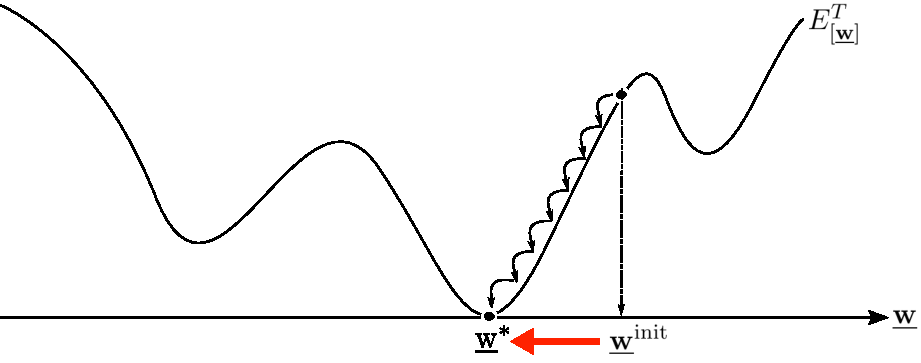
\includegraphics[trim=150 0 0 0,clip,height=2.5cm]{img/section1_fig19}}%
     \begin{subfigure}[t]{0.35\textwidth}
         \centering
         \usebox{\imagebox}% Place largest image
     \end{subfigure}
     \hspace{7mm}
     \begin{subfigure}[t]{0.49\textwidth}
         \centering
         \raisebox{\dimexpr.5\ht\imagebox-.5\height}{% Raise smaller image into place
         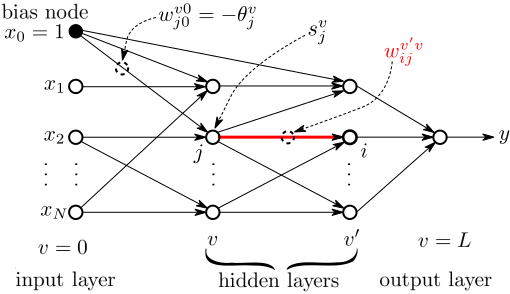
\includegraphics[width=0.99\textwidth]{img/section1_fig14_ij}
         }
     \end{subfigure}
    \end{figure}
    }
\end{frame}

\begin{frame}
    
    \begin{figure}[h]
        \centering
        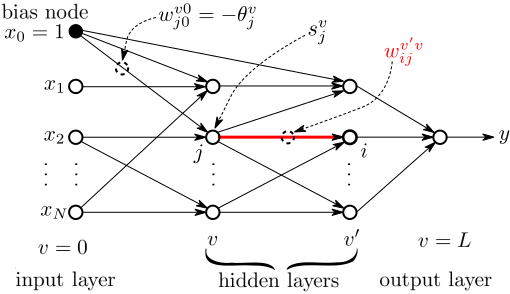
\includegraphics[height=3cm]{img/section1_fig14_ij}
        \caption{Example MLP architecture}
    \end{figure}
    
    \mode<article>{
    \eqref{eq:gradient_descent_mlp} shows us how gradients are used for iteratively finding the minimum of the training error.
    The layered structure of an MLP implies that computing the gradient requires a more involved application of the chain rule.
    }
    
    
    
\end{frame}

\mode*

\newpage

\mode<all>
\section{The Backpropagation algorithm}

\definecolor{darkgreen}{rgb}{0,0.6,0}
\definecolor{darkcyan}{rgb}{0,0.5,0.5}
\definecolor{darkyellow}{rgb}{0.5,0.5,0}
\definecolor{mangenta}{rgb}{1,0,1}

\begin{frame}\frametitle{\secname}

The Backpropagation algorithm is a method for computing gradients by using the chain rule efficiently.
\mode<article>{\eqref{eq:gradient_terms} shows us how the gradient breaks down into (1) an error term and (2) a term dependent on the type of model chosen. Specifically:
}	
\begin{equation}
	\textcolor{orange}{	\frac{\partial y(\vec{x}; \vec{w})}{
			\partial {w}_{ij}^{v'v}}}
    \label{eq:model_term}
\end{equation}
\mode<article>{
The Backpropagation algorithm handles the computation of the term in \eqref{eq:model_term} for neural networks such as the one depicted in \figref{fig:example_mlp}.
}
\end{frame}

% -----------------------------------------------------------------------------
\begin{frame} \frametitle{Gradients in neural networks}
    
    \mode<article>{
    The Backpropagation algorithm is not tied to any specific neural architecture. We will therefore attempt to formulate how it works in the general sense.\\
    
    Let $w^{v'v}_{ij}$ be the weight connecting neuron $j$ in layer $v$ to neuron $i$ in layer $v'$, In order to compute $\frac{\partial y(\vec{x}; \vec{w})}{
			\partial {w}_{ij}^{v'v}}$ we need to identify the following:
    \begin{itemize}
        \item $P(v, j)$: the set of immediate parent nodes feeding input into neuron $(v, j)$,
        \item $C(v', i)$: the set of immediate children nodes which neuron $(v', i)$ provides with input
    \end{itemize}
    }
    
    \begin{figure}[h]
    \centering   
    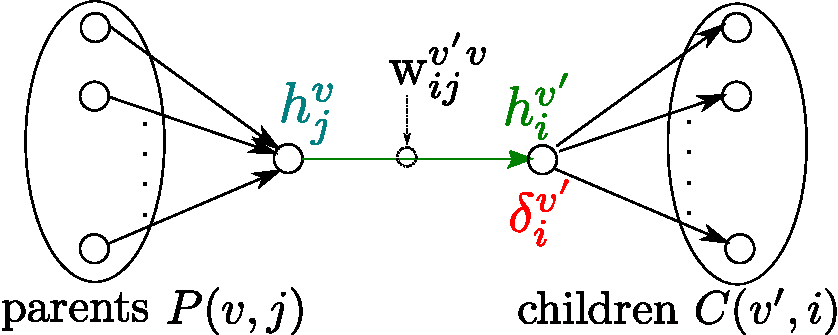
\includegraphics[height=3cm]{img/section1_fig20_mini_multicolor.pdf}
    \mode<article>{
    \caption{Nodes $(v,j)$ and $(v', i)$ are directly connected via the weight $w^{v'v}_{ij}$. The bias node for neuron $(v,j)$ is included in the set of its parent nodes.}
    }
    \label{fig:connection_ij}
    \end{figure}
    
    \mode<article>{
    $h^{v'}_{i}$ measures the total input arriving at neuron $i$ in layer $v'$.
    $h^{v'}_{i}$ is the weighted sum of this neuron's parent activations:
    }
    
    \mode<presentation>{\vspace{-5mm}
    }
    \begin{equation}
            {\color{darkgreen}h_i^{v'}} 
            := 
            \kern-2ex
            \sum_{(\mu,k) \in P(v',\,i)}
            \kern-2ex
            w_{ik}^{v'\mu}\; 
            f_k^\mu\big( {\color{teal} h_k^\mu} \big)   
            \label{eq:total_input_vi},
    \end{equation}
    
    \mode<article>{
    where $\mu$ and $k$ in \eqref{eq:total_input_vi} serve as indices for describing the position of each parent node in $P(v', i)$ in the network.
    }
    \mode<presentation>{\vspace{-5mm}
    }
    
    \pause 
    \question{How does $w_{ij}^{v'v}$ contribute to the error?
    \slidesonly{$\frac{\partial y(\vec{x}; \vec{w})}{\partial w_{ij}^{v'v}} = \ldots$
    \pause
    }}\\
    
    \mode<article>{
    - The contribution is measured by applying the chain rule:
    }
    \mode<presentation>{\vspace{-9mm}
    }
    
    \begin{eqnarray}
        \frac{\partial y(\vec{x}; \vec{w})}{\partial w_{ij}^{v'v}}
            = \underbrace{\frac{\partial y(\vec{x}; \vec{w})}
                {{\color{darkgreen}\partial h_i^{v'}}} }_{ 
                    \substack{\coloneqq\;{\color{red}\delta_i^{v'}} \\
                    \text{``local error''} \\
                    \text{at neuron} \\
                    (v', i)}
                }
              \cdot 
              \underbrace{\frac{{\color{darkgreen}\partial h_i^{v'}}}
                {\partial w_{ij}^{v'v}}}_{
                    \substack{=\;f_j^v({\color{teal} h_j^v}) \\
                    \text{activity} \\
                    \text{of neuron} \\
                    (v, j)}}
                \label{eq:input_output_terms}
    \end{eqnarray}
    
    \mode<article>{
    \eqref{eq:input_output_terms} breaks the contribution of  $w_{ij}^{v'v}$ to the network's output into two parts:
    \begin{enumerate}
     \item The contribution of $h^{v'}_{i}$ to the network's response $y(\vec x; \vec w)$. This is referred to as the ``local error'' at neuron $(v',i)$. The efficiency of the Backpropagation algorithm is based on how it computes the ``local error'' denoted by $\delta_i^{v'}$ for neuron $(v', i)$ and all other neurons in the network.
     \item The contribution of $h^{v'}_{i}$ due to one of its inputs, namely neuron $(v,j)$ which is weighted by $w_{ij}^{v'v}$. We already have everything to compute this term and that is by taking the definition of $h^{v'}_{i}$ in \eqref{eq:total_input_vi} and taking the derivative w.r.t. $w_{ij}^{v'v}$. 
     This should be straightforward since only a single term in the sum depends on $w_{ij}^{v'v}$:
         \begin{equation}
            \frac{{\color{darkgreen}\partial h_i^{v'}}}
            {\partial w_{ij}^{v'v}}
            =  \frac{\partial}
            {\partial w_{ij}^{v'v}}
            \left(
            \sum_{(\mu,k) \in P(v',\,i)}
            \kern-3ex
            w_{ik}^{v'\mu}\; 
            f_k^\mu\big( {\color{teal} h_k^\mu} \big){}
            \right)
            = \underbrace{f_j^v({\color{teal} h_j^v})}_{
            \substack{
                    \text{activity} \\
                    \text{of neuron} \\
                    (v, j)
                    }}
        \end{equation}
    \end{enumerate}
    }
\end{frame}

\begin{frame}\frametitle{The Backpropagation algorithm}
    The Backpropagation algorithm is composed of two stages:
    \begin{enumerate}
     \item \textbf{forward propagation} (forward pass)
     \mode<article>{: Given some input $\vec x$, compute the activities of all neurons and the response of the network.}
     \item \textbf{backward propagation} (backward pass)
     \mode<article>{: Given the response of the network, recursively calculate the local errors starting with the output node and work your way backward through the network.}
    \end{enumerate}
\end{frame}

\subsection{Forward and backward propagation}

% -----------------------------------------------------------------------------
\begin{frame} \frametitle{The Backpropagation algorithm}
    \mode<presentation>{
	\only<1,2>{\placeimage{9.5}{1}{img/section1_fig20_mini_multicolor.pdf}{width=4.8cm}}
	\only<3->{\placeimage{9.5}{1}{img/section1_fig20_mini_back_multicolor.pdf}{width=4.8cm}}
    }
    \mode<presentation>{ \vspace{11mm} }
	\begin{enumerate}
		\item \textbf{forward propagation}: calculate activities 
				$f_i^{v'}({\color{darkgreen}h_i^{v'}})$
				{\small(parents $\rightarrow$ children)}
				$$	
					{
					%\color{darkgreen}
					h_j^0
					} 
						\;:=\; \mathrm{x}_j \,, 
					\quad 
					{\color{darkgreen}h_i^{v'}}
		   			\,= \kern-2ex\smallsum{(\mu,k) \in P(v',\,i)}{} \kern-2ex
	   			w_{ik}^{v'\mu}\;  f_k^\mu\big( {\color{teal} h_k^\mu} \big) \,,
					\quad
					y(\vec{x}; \vec{w})\,=\, f_1^L({\color{blue}h_1^L})
				$$\\\vspace{-2mm}
	\only<1>{	
		\mode<presentation>{
		\begin{center}
		\vspace{2mm}
		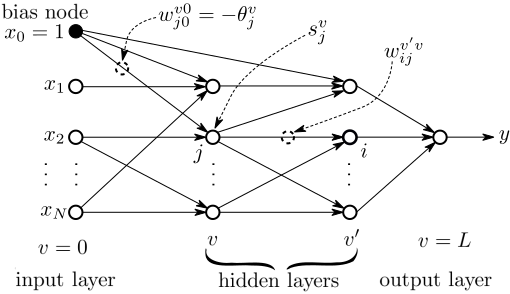
\includegraphics[height=4cm]{img/section1_fig14}
		\end{center}
		}
	}
	\only<2>{	
		\mode<presentation>{
		\begin{center}
		\vspace{2mm}
		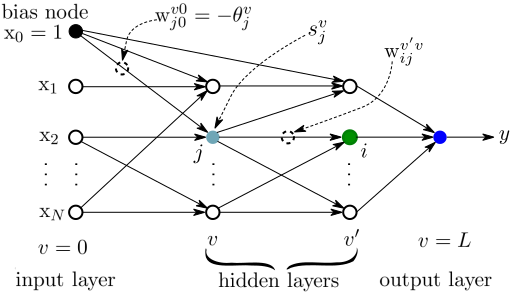
\includegraphics[height=4cm]{img/section1_fig14_fwd}
		\end{center}
		}
	}
	\only<3->{
		\item \textbf{backpropagation}: calculate ``local errors'' 
				$\color{red}\delta_i^{v'}$
				{\small(children $\rightarrow$ parents)}
				\vspace{-1mm}
				%~ \begin{eqnarray*} 
				%~ \end{eqnarray*}
				\begin{eqnarray} 
				{\color{red} \delta_1^L}
				&=& \frac{\partial y(\vec{x}; \vec{w})} {{\color{blue}\partial h_1^{L}}}
					= [f_1^{L}]'({\color{blue} h_1^{L}})
							%\;\;\text{for}\;v'=L
							\\
					{\color{red}\delta_i^{v'}} 
					\only<3>{
						&=&  \frac{\partial y(\vec x; \vec w)}{\color{darkgreen}\partial h^{v'}_{i}}
						\qquad \text{``local error'' at neuron }(v', i)
                        \label{eq:delta_step1}\\
						}
					\only<4->{
						&=&  \kern-3ex\sum\limits_{(v''\hspace{-1mm},\,k) \in C(v',\,i)}{
						\underbrace{
							\smallfrac{\partial y(\vec{x}; \vec{w})}
								{{\color{blue}\partial  h_k^{v''}}}
							}_{{\color{red}\delta_k^{v''}}} 
						\;\kern1.5ex\cdot \kern-2.5ex\;
						\underbrace{\smallfrac
								{{\color{blue}\partial h_k^{v''}} }
								{{\color{darkgreen}\partial h_i^{v'}}}
							}_{{w}_{ki}^{v''v'} \kern-.5ex\cdot\kern.5ex
								[f_i^{v'}]'({\color{darkgreen}h_i^{v'}}) }}
                            \label{eq:delta_step2}
                                \notesonly{\\&=&  \kern-3ex\sum\limits_{(v''\hspace{-1mm},\,k) \in C(v',\,i)}{
						{\kern-2ex {\color{red}\delta_k^{v''}}}
                        \cdot\,
						{{w}_{ki}^{v''v'} \kern-.5ex\kern.5ex
								[f_i^{v'}]'({\color{darkgreen}h_i^{v'}}) }}}
                                \notesonly{\\ \kern-3ex&=&\;\;\; }%\,,
                                \slidesonly{\kern-3ex=\;\;\; }%\underbrace{
							[f_i^{v'}]'({\color{darkgreen}h_i^{v'}}) 
							\kern-3ex\sum_{(v''\hspace{-1mm},\,k) \in C(v',\,i)}\kern-3ex
							{\color{red}\delta_k^{v''}} 
							{w}_{ki}^{v'' v'} 
						}
						%}_{{\color{red} \delta_i^L}\;=\;
						%	[f_i^{L}]'({\color{darkgreen} h_i^{L}})
						%	\;\;\text{for}\;v'=L}
				\end{eqnarray}
		}
		\only<5->{
		\vspace{-1mm}
		\item[] \textbf {weight update}: using activities and local errors
        \begin{equation}
				{w}_{ij}^{v'v}
				\; \leftarrow \; 
				{w}_{ij}^{v'v} - \eta \cdot
				\smallfrac{\partial e}{\partial{w}_{ij}^{v'v}}
				\;=\; {w}_{ij}^{v'v} - \eta \, \cdot 
				\smallfrac{\partial e}{\partial y(\vec{x}; \vec{w})} \cdot
				\only<5>{
				\smallfrac{\partial y(\vec{x}; \vec{w})}{\partial{w}_{ij}^{v'v}}\hspace{8.5mm}
				}
                \slidesonly{
				\only<6>{
				{\color{red} \delta_i^{v'}} \kern-.5ex\cdot
			   			f_j^v( {\color{teal}h_j^v} )
			   	}}
        \end{equation}
        \notesonly{
        \begin{equation}
				{w}_{ij}^{v'v}
				\quad \leftarrow \quad 
                {w}_{ij}^{v'v} - \eta \, \cdot
				\smallfrac{\partial e}{\partial y(\vec{x}; \vec{w})} \cdot
				{
				{\color{red} \delta_i^{v'}} \kern-.5ex\cdot
			   			f_j^v( {\color{teal}h_j^v} )
			   	}
        \end{equation}
        }
			}
	\end{enumerate}
	%{\scriptsize
	%Computational complexity: $O(n)$, $n$: number of weights \& thresholds}
    
\end{frame}

\mode<article>{
    To understand how the ``local error'' at neuron $(v',i)$ goes from its definition in \eqref{eq:delta_step1} to \eqref{eq:delta_step2}, one needs to look at the propagation from $(v',i)$ forwards to all its immediate children nodes in $C(v', i)$. Let $(v'', k)$ describe a neuron positioned deeper in the network and connected to $(v',i)$, making it one of its children and, in turn, making $(v',i)$ one of the parents of $(v'', k)$.\\
    Analogous to how we compute in ${\color{darkgreen}h_i^{v'}}$ in \eqref{eq:total_input_vi}:
    
    \begin{align}
            {\color{blue}h_k^{v''}} 
            :=& 
            \kern-2ex
            \sum_{(\mu,\,l) \in P(v'',\,k)}
            \kern-2ex
            w_{kl}^{v''\mu}\; 
            f_l^\mu\big( {h_l^\mu} \big)   
            \label{eq:total_input_vddk}\\
            =&\; \ldots \,+\,{}
            w_{ki}^{v''v'}\; 
            f_i^{v'}\big( {\color{darkgreen}h_i^{v'}})
            \,+\, \ldots
    \end{align}
    
    Since only one term in this sum depends on ${\color{darkgreen} h_i^{v'}}$:
    \begin{align}
    \frac{{\color{blue}\partial h_k^{v''}} }{{\color{darkgreen}\partial h_i^{v'}}}
    \;&= \;
    \frac{\partial}{\color{darkgreen}\partial h_i^{v'}}
    \left(
    w_{ki}^{v''v'}\; 
            f_i^{v'}\big( {\color{darkgreen}h_i^{v'}})
    \right)\\
    \;&= \; w_{ki}^{v''v'} \,
    \frac{\partial}{\color{darkgreen}\partial h_i^{v'}}
            f_i^{v'}\big( {\color{darkgreen}h_i^{v'}})\\
    \;&= \; {{w}_{ki}^{v''v'} \;
    [f_i^{v'}]'({\color{darkgreen}h_i^{v'}}) }
    \end{align}
}

\clearpage

\subsection{Example: MLP with fully connected layers}

\mode<article>{
We will apply the Backpropagation algorithm to an MLP as depicted by \figref{fig:mlp_fc}. All neurons in one layer are connected with all nodes of the next layer. The layers are therefore \emph{fully connected}. This implies that the weights between consecutive layers make up a \emph{dense} weight matrix. This allows us to express the formulas using vector notation.  
}

\begin{frame}\frametitle{\subsecname}
    \begin{figure}[h]
    \centering   
    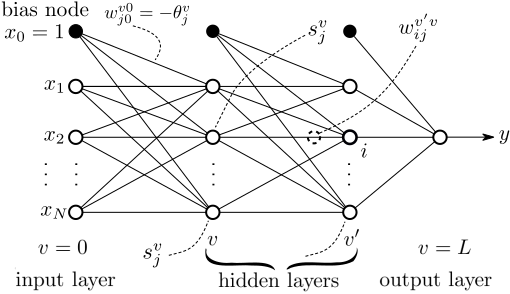
\includegraphics[height=5cm]{img/section1_fig14_fc}
    \mode<article>{
    \caption{MLP with fully connected layers}
    }
    \label{fig:mlp_fc}
    \end{figure}
    
\notesonly{Recall that the purpose of the Backpropagation algorithm is to compute the gradients. Therefore, the task is to obtain an expression for computing }\slidesonly{compute} the gradients for all weights and biases in this network:\\

\pause

\question{What is the procedure for the Backpropagation algorithm?}\\

\mode<article>{
- The procedure is:
\begin{enumerate}
 \item forward pass: compute ${h^{v}_{i}}$ for $v = 0,\ldots,L$,\\
 \item backward pass: backpropagation of ``local errors'' (i.e. compute ${\color{red}\delta^{v}_{i}}$).
\end{enumerate}
}
\end{frame}

\subsubsection{The forward pass}
\begin{frame}\frametitle{\subsubsecname}
    
    \mode<presentation>{
    \placeimage{7.4}{1}{img/section1_fig14_fc_nolayers}{width=6.7cm}
    \begin{textblock}{4}(0.5,2)
    \begin{equation}
    \boxed{
        {\color{darkgreen}h_i^{v'}}
        \,= \kern-2ex
        \smallsum{(\mu,k) \in P(v',\,i)}{}
        \kern-2ex
        w_{ik}^{v'\mu}\; f_k^\mu\big( {\color{teal} h_k^\mu} \big)
    }
    \end{equation}
    \end{textblock}
    \vspace{1cm}
    }
    
    Compute ${h^{v}_{i}}$ \only<1>{for $v = 0,\ldots,L$}:

    \begin{itemize}
    \only<1,2>{
        \item $v=0$ (input layer):\\ \slidesonly{\vspace{-3mm}}
        \begin{flalign}
            h^{0}_{j} &=
            \slidesonly{\only<1>{&&}}
            \only<2>{
                              x_{j}\;,   & j=1,\ldots,N&&\\
                h^{0}_{0}  &=  x_{0} = 1          & (\text{bias node})\\
                \vec h^{0} &= \vec x     & (\text{bias included})\\
                f^0_{j}(h) :\kern-0.5ex&= h & \text{ (identity function)}\\
                %\Rightarrow\; 
                \vec f^0(\vec h) &= \vec x & \text{ (identity, bias included)}
            }
        \end{flalign}
    }
    \only<3,4>{
        \slidesonly{\vspace{5mm}}
        \item $v=1$ (1\textsuperscript{st} hidden layer with $N_{1} \text{ nodes}$):\\ \slidesonly{\vspace{-2mm}}
        \begin{flalign}
        h^{1}_{j} &= 
        \slidesonly{\only<3>{&&}}
        \only<4>{
            \smallsum{k=0}{N} w_{jk}^{10}\;  f_k^0\big( {h_k^0} \big) = {\vec w_{j}^{10}}^{\top} \vec h^0 & (\text{bias included})&&\\
            \vec h^{1} &= {\vec W^{10}}^{\top} \vec h^0 = {\vec W^{10}}^{\top} \vec x &(\text{biases included})\\
            f^1_{j}(h) :\kern-0.5ex&= \text{e.g. }\tanh(h),  &j=1,\ldots,N_{1}\\ f^1_{0}(h) :\kern-0.5ex&= h &\text{(identity for bias)}\\
        }
        \end{flalign}
    }
    \only<5,6>{
        \item $v=2$ (2\textsuperscript{nd} hidden layer with $N_{2} \text{ nodes}$):\\ \slidesonly{\vspace{-7mm}}
    % temporarily change footnote marks to symbols so not to confuse with exponents
    %\renewcommand*{\thefootnote}{\fnsymbol{footnote}}
        \begin{flalign}
        h^{2}_{i} &=
        \slidesonly{\only<5>{&&}}
        \only<6>{
            \smallsum{j=0}{N_{1}} w_{ij}^{21}\;  f_j^1\big( {h_j^1} \big) = 
            {\vec w_{i}^{21}}^{\top} 
            %\overbrace{
            \vec f^{1}(\vec h^1)
            %}^{
            %\vec s^1
            %} 
            &(\text{bias included})&&\\
            \vec h^{2} &= {\vec W^{21}}^{\top} \vec f^{1}(\vec h^1) &(\text{biases included})\\
            f^2_{i}(h) :\kern-0.5ex&= \text{e.g. }\tanh(h) &i=\mathbf{1},\ldots,N_{2}\\
            f^2_{0}(h) :\kern-0.5ex&= h &\text{(identity for bias)}\\
        }
        \end{flalign}
        }
    \only<7,8>{
        \item $v=L$ (output layer):\\ \slidesonly{\vspace{-4mm}}
        \begin{flalign}
        h^{L}_{1} &=
        \slidesonly{\only<7>{&&}}
        \only<8>{
            \smallsum{i=0}{N_{2}} w_{1i}^{L2}\;  f_i^1\big( {h_i^1} \big) = {\vec w_{1}^{21}}^{\top} \vec f^{2}(\vec h^2) &(\text{bias included})&&\\
            y(\vec x; \vec w) &= f^L_{1}(h^{L}_{1})&&\\
            f^L_{1}(h) :\kern-0.5ex&= \text{e.g. logistic function (sigmoid)}\\
        }
        \end{flalign}
    }
    \end{itemize}
    
\end{frame}

\subsubsection{The backward pass}

\begin{frame}\frametitle{\subsubsecname}
    \mode<presentation>{
    \placeimage{7.4}{1}{img/section1_fig14_fc_nolayers}{width=6.7cm}
    \begin{textblock}{4}(0.5,2)
    \begin{equation}
    \boxed{
        {\color{red}\delta_i^{v'}}
        =
        [f_i^{v'}]'({\color{darkgreen}h_i^{v'}}) 
        \kern-3ex\sum_{(v''\hspace{-1mm},\,k) \in C(v',\,i)}\kern-3ex
        {\color{red}\delta_k^{v''}} 
        {w}_{ki}^{v'' v'}
            }
    \end{equation}
    \end{textblock}
    \vspace{2cm}
    }
    
    Compute ${\color{red}\delta^{v}_{i}}$:
    
    % temporarily change footnote marks to symbols so not to confuse with exponents
    \renewcommand*{\thefootnote}{\fnsymbol{footnote}}
    \begin{itemize}
    \only<1,2>{
        \item $v=L$ (output layer):\\ \slidesonly{\vspace{-4mm}}
        \begin{flalign}
            y(\vec x; \vec w) &= f^L_{1}(h^{L}_{1})&&\\
            f^L_{1}(h) &= \text{e.g. logistic function (sigmoid)}\\
            {\color{red}\delta^{L}_{1}}  &= \frac{\partial y(\vec{x}; \vec{w})} {{\color{blue}\partial h_1^{L}}} =
        \only<2>{
                [f_1^{L}]'({\color{blue} h_1^{L}})
        }
        \end{flalign}
    }

    \only<3,4>{
        \item $v=2$ (2\textsuperscript{nd} hidden layer with $N_{2} \text{ nodes}$):\\ \slidesonly{\vspace{-7mm}}
        \begin{flalign}
            f^2_{i}(h) :\kern-0.5ex&= \text{e.g. }\tanh(h), &i=1,\ldots,N_{2}&&\\
            f^2_{0}(h) :\kern-0.5ex&= h &\text{(identity for bias)}\\
            {\color{red}\delta^{2}_{i}} &=
        \only<4>{
                [f_i^{2}]'({\color{darkgreen}h_i^{2}})\;
                {\color{red}\delta_1^{L}} \,
                {w}_{1i}^{L2}
                &(\text{bias }{\scriptsize{w}_{0i}^{L2}}\text{ excl.})\\
             {\color{red} \vec \delta^{2}} &=\; [\vec f^{2}]'({\color{darkgreen}\widetilde{\vec h}^{2}}) \odot ({\color{red}\delta_1^{L}} \cdot {\widetilde{\vec w}_{1}^{L2}})
        \notesonly{ \footnotemark }
        %\notesonly{ \footnotemark }
        }
        \end{flalign}
        \notesonly{
            \footnotetext{
            $\widetilde{\vec {w}}_{1}^{L2} \; \corresponds \; {\vec {w}}_{1}^{L2}$ without the bias node.\\
            ${\color{darkgreen} {\vec{\widetilde{h}}^{2}}}  \; \corresponds \; {\color{darkgreen} {\vec{{h}}^{2}}}$ without the bias node.
            ``$\odot$'' stands for elementwise multiplication, while ``$\cdot$'' stands for the dot product.
            }
        }
        %\notesonly{
        %\footnotetext{``$\odot$'' stands for elementwise multiplication, while ``$\cdot$'' stands for the dot product.}
        %}
        }
    \only<5,6>{
        \item $v=1$ (1\textsuperscript{st} hidden layer with $N_{1} \text{ nodes}$):\\ \slidesonly{\vspace{-5mm}}
        \begin{flalign}
            f^1_{j}(h) :\kern-0.5ex&= \text{e.g. }\tanh(h),  &j=1,\ldots,N_{1}\\ f^1_{0}(h) :\kern-0.5ex&= h &\text{(identity for bias)}&&\\
            {\color{red}\delta^{1}_{j}}
             &=
        \only<6>{
                [f_j^{1}]'({\color{darkgreen}h_j^{1}}) 
                \kern-.5ex\sum_{k=1}^{N_{2}}\kern-.5ex
                {\color{red}\delta_k^{2}} \,
                {w}_{{\color{magenta}kj}}^{21} %\\%&
                %\notesonly{\\&}
                %= 
                %[f_j^{1}]'({\color{darkgreen}h_j^{1}})\,
                %{\color{red} {\vec{\widetilde{\delta}}^{2}}^{\top}}
                %\widetilde{\vec {w}}_{j}^{21}
                &(\text{bias k=0  excl.})\\%TODO: vector notation for this
                %\notesonly{\\[3mm]}\slidesonly{\\}
                %(\text{skip }k=0)\\
                %}
        %\end{flalign}
        %\vspace{-2mm}
        %\begin{flalign}
        %\only<6>{
            {\color{red} \vec \delta^{1}}
             &=
                [\vec f^{1}]'({\color{darkgreen}\widetilde{\vec h}^{1}})
                \odot
                (
                \kern-.5ex\cdot
                \widetilde{\vec {W}}^{21}
                {\color{red} {\vec \delta^{2}}}) \notesonly{ \footnotemark }
                & \\
             %&= 
                %[\vec f^{1}]'({\color{darkgreen}h^{1}})
                %\odot
                %({{\vec {\widetilde{W}}}^{21}}^{\top} 
                %\kern-.7ex\cdot
                %{\color{red} {\vec{\widetilde{\delta}}^{2}}^{\top}})
                %& (\vec A\, \vec B)^{\kern-.5ex\top}\kern-1ex=\vec B^{\top}\kern-.8ex\vec A^{\kern-.5ex\top}
        }
        \end{flalign}
        \notesonly{
            \footnotetext{
            $\widetilde{\vec {W}}^{21} \; \corresponds \; {\vec {W}}^{21}$ without the bias in each column vector ${\vec {w}}_{j}^{21}$. $w_{\color{magenta}{kj}}^{21}$ refers to row ${\color{magenta}j}$, col. ${\color{magenta}k}$ of $\widetilde{\vec {W}}^{21}$.
            ${\color{darkgreen} {\vec{\widetilde{h}}^{1}}}  \; \corresponds \; {\color{darkgreen} {\vec{{h}}^{1}}}$ without the bias node.
            %${\color{red} {\vec{\widetilde{\delta}}^{2}}^{\top}}  \; \corresponds \; {\color{red} {\vec{{\delta}}^{2}}^{\top}}$ without the bias node (k=0), i.e. ${\color{red} {\vec{\widetilde{\delta}}^{2}}^{\top}}$ is ${\color{red} {\vec{{\delta}}^{2}}^{\top}}$ without ${\color{red} \delta^{2}_{0}}$.
            }
        }
    }
    \only<7,8>{
        \item $v=0$ (input layer):\\ \slidesonly{\vspace{-3mm}}
        \begin{flalign}
                f^0_{j}(h) :\kern-0.5ex&= h & \text{ (identity function)}&&\\
                \vec f^0(\vec h) :\kern-0.5ex&= \vec x &\text{ (bias included)}
                \\
            {\color{red}\delta^{0}_{j}}
             &\;
            \only<8>{
            &
             (\text{Not applicable to observed input})
             }
        \end{flalign}
        \slidesonly{
        \vspace{5mm}
        \begin{equation}
		\boxed{
				{w}_{ij}^{v'v}
				\, \leftarrow \, 
				{w}_{ij}^{v'v} - \eta \cdot
				\smallfrac{\partial e}{\partial y(\vec{x}; \vec{w})} \cdot
				\smallfrac{\partial y(\vec{x}; \vec{w})}{\partial{w}_{ij}^{v'v}}
				\;=\; {w}_{ij}^{v'v} - \eta \cdot
				\smallfrac{\partial e}{\partial y(\vec{x}; \vec{w})} \cdot
				{\color{red} \delta_i^{v'}} \kern-.5ex\cdot
			   			f_j^v( {\color{darkgreen}h_j^v} )
		}
        \end{equation}
        }
    }
    \end{itemize}
    % change footnote marks back to original scheme (numbers)
    \renewcommand*{\thefootnote}{\arabic{footnote}}
    
\end{frame}

\begin{frame}

{\renewcommand{\arraystretch}{1.5} %<- control vertical spacing
\begin{table}[!h]
\centering
\caption{Overview of dimensions}
%\resizebox{\textwidth}{!}
{%
\label{tab:summary_bp} 
\begin{tabular}{|c||c|c|c|}
\hline
\multicolumn{1}{|c||}{layer} & \multicolumn{1}{c|}{parameters}                  & \multicolumn{1}{c|}{total input} & \multicolumn{1}{c|}{``local'' errors}\\ 
\hline \hline
$v=0$
& N/A 
&
\begin{tabular}[c]{@{}l@{}}
    $\vec h^{0} := \vec x$\\
    $\vec h^{0} \in \R^{N+1}$\vspace{2mm}
\end{tabular} 
& N/A\\ 
\hline
$v=1$ 
& \begin{tabular}[c]{@{}l@{}}
    $\vec w_{j}^{10}  \in \R^{N+1}$\\
    $\vec {W}^{10} \in \R^{(N+1) \times N_{1}}$\vspace{2mm}
\end{tabular} 
& \begin{tabular}[c]{@{}l@{}}
    %$\vec h^{1} := \vec f({\vec {W}^{10}}^{\top}\vec x)$\\
    $\vec h^{1} \in \R^{N_{1}+1}$\\
    $\widetilde{\vec h}^{1} \in \R^{N_{1}}$\vspace{2mm}
\end{tabular} 
& \begin{tabular}[c]{@{}l@{}}
    ${\color{red} \vec{\delta}^{1}} \in \R^{N_{1}}$\vspace{2mm}
\end{tabular} \\ 
\hline
$v=2$ 
& \begin{tabular}[c]{@{}l@{}}
    $\vec w_{i}^{21}  \in \R^{N_{1}+1} $\\
    $\vec {W}^{21}  \in \R^{(N_{1}+1) \times N_{2}}$\\
    $\widetilde{\vec {W}}^{21}  \in \R^{(N_{1}) \times N_{2}}$\vspace{2mm}
\end{tabular} 
& \begin{tabular}[c]{@{}l@{}}
    $\vec h^{2} \in \R^{N_{2}+1}$\\
    $\widetilde{\vec h}^{2} \in \R^{N_{2}}$\vspace{2mm}
\end{tabular}
& \begin{tabular}[c]{@{}l@{}}
    ${\color{red} \vec{\delta}^{2}} \in \R^{N_{2}}$ \\
    %${\color{red} \widetilde{\vec{\delta}}^{2}} \in \R^{N_{2}}$\vspace{2mm}
\end{tabular} \\ 
\hline
$v=L$ 
& \begin{tabular}[c]{@{}l@{}}
    $\vec w_{1}^{L2}  \in \R^{N_{2}+1}$\vspace{2mm}
\end{tabular} 
& $h_1^{L} \in \R$ 
& ${\color{red}\delta^{L}_{1}} \in \R$\\ 
\hline
\end{tabular}
}
\end{table}
} % arraystretch
    
\end{frame}

\clearpage

% -----------------------------------------------------------------------------
\definecolor{forward}{rgb}{0,0.7,0}
\definecolor{backward}{rgb}{0.8,0,0}

\subsection{Summary of the Backpropagation for gradient descent}

\begin{frame} \frametitle{\subsecname}
    \mode<presentation>{
	\only<1>{
		\placeimage{10.75}{5.5}{img/MLP_forward.pdf}{width=3.75cm}
		\placeimage{10.75}{8.7}{img/MLP_backward.pdf}{width=3.75cm}
	}}
	
	%\begin{algorithm}[H] 
		%\scriptsize
		\footnotesize
		\DontPrintSemicolon
		initialization of weights and thresholds \\
        
		\While{stopping criterion not met}{
			$\text{gradient}_{ij}^{v'v} := 0 
					\,, \quad \forall w_{ij}^{v'v}$ \\
                    
			\For{$\alpha \in \{1,\ldots,p\}$}{
				${\color{forward}h_i^0} 
					:= x_i^{(\alpha)} \,, \quad \forall i$ 
				\qquad\qquad // {\color{forward}forward propagation}\\
                
				\For{$v' \in \{1,\ldots,L\}$}{
					%~ ${\color{forward} h_i^{v'}} 
						%~ := \sum\limits_{\scriptscriptstyle
							%~ (v',i) \in C(v,j)} w_{ij}^{v'v} 
							${\color{forward}h_i^{v'}}
		   			\;\;=\;\; \kern-2ex\smallsum{(\mu,k) \in P(v',i)}{} \kern-2ex
	   			w_{ik}^{v'\mu}\;  \underbrace{f_k^\mu\big( {\color{forward} h_k^\mu} \big) 
								%~ \underbrace{f_j^v({\color{forward} h_j^{v}})
								}_{\kern-2exx_k^{(\alpha)} \;\text{if}\; 
									v'=1\kern-2ex } \,,
							\quad \forall i$
					\vspace{-1.5mm}
				}
				${\color{backward} \delta_1^L} 
					:= [f_1^L]'({\color{forward}h_1^L}) $%\,, \quad \forall i$ 
				\qquad // {\color{backward}backward propagation}\\
                
				\For{$v' \in \{L-1,\ldots,1\}$} {
					${\color{backward}\delta_i^{v'}} 
						:= [f_{i}^{v'}]'({\color{forward}h_i^{v'}}) 
						\kern-1ex\sum\limits_{(\mu,k) \in C(v',i)}\kern-1ex
						{\color{backward} \delta_k^{\mu}} 
						\, w_{ki}^{\mu v'} \;,
						\quad \forall i$
					\vspace{-2.5mm}
				}
				$\text{gradient}_{ij}^{v'v} := \text{gradient}_{ij}^{v'v}
						+ \frac{\partial e^{(\alpha)}}{\partial y(\vec x; \vec w)}
						 \, {\color{backward}\delta_i^{v'}} 
						 \, f_j^v({\color{forward}h_j^v})
						 \,, \quad \forall w_{ij}^{v'v}$
				\hspace{11mm} // sum
			}
			\notesonly{ // gradient descent step:\\
            
            }
			$\text{gradient}_{ij}^{v'v} := \frac{1}{p} \text{gradient}_{ij}^{v'v}$\\
			% $w_{ij}^{v'v} := w_{ij}^{v'v} - \frac{\hat \eta}{p}
			 $w_{ij}^{v'v} := w_{ij}^{v'v} - \eta
					\, \text{gradient}_{ij}^{v'v} 
					\,, \quad \forall w_{ij}^{v'v}	$
			\slidesonly{\hspace{15mm} // gradient descent step}
					\vspace{-1.5mm}
		}
		%\caption{Backpropagation in feedforward networks}
	%\end{algorithm}
\end{frame}

\subsubsection{Complexity}

\begin{frame}\frametitle{\subsubsecname}

The computational and 
memory complexity of the Backpropagation algorithm is
$\mathcal{O}(n)$, %\quad,{}
where $n$ is the total number of the weights in the network. 
\mode<article>{It is therefore, 
\emph{linear} in the 
number of weights.}

An alternative\slidesonly{:}\notesonly{and very simple method for computing the gradients would be to use }
\pause
\emph{finite differences}.

Let $\widetilde{\vec w}$ denote all parameters of the network except for a single weight $w^{v'v}_{ij}$

\mode<article>{
The idea is to add (subtract) a small offset $\varepsilon$ to (from) $w^{v'v}_{ij}$ in the network, while keeping all other weights $\widetilde{\vec w}$ fixed and measure the change in the error function. Specifically,
}
\begin{equation}
e\big(y_T, y\big(\vec x; \widetilde{\vec w}, {w}^{v'v}_{ij} \pm \varepsilon\big)\big) =: e\big(\widetilde{\vec w}, {w}^{v'v}_{ij} \pm \varepsilon\big) \text{ for brevity}
\end{equation}
\pause
For $\varepsilon \ll 1$ follows:

\begin{equation}
\frac{\partial e\left(y_T, y\left(\vec x; {\vec w}\right)\right)}{\partial {w}^{v'v}_{ij}} =
\frac{
e\big(\widetilde{\vec w}, {w}^{v'v}_{ij} + \varepsilon\big)
+
e\big(\widetilde{\vec w}, {w}^{v'v}_{ij} - \varepsilon\big)
}
{2 \,\varepsilon}
+ \mathcal{O}(\varepsilon^{2})
\label{eq:finitediff}
\end{equation}

\notesonly{
The complexity of the forward propagation remains $\mathcal{O}(n)$. Performed it twice in \eqref{eq:finitediff} is manageable as $\mathcal{O}(2n) \leadsto \mathcal{O}(n)$.
However, this is the complexity for a single weight. Performing this for all $n$ weights in the network increases the complexity of finite differences to $\mathcal{O}(n^{2})$.

However, numerical differentiation such as finite differences remains a useful tool for debugging your Backpropagation algorithm and performing gradient checks.
}

\pause

\slidesonly{
Complexity of finite differences increases to.$\mathcal{O}(n^{2})$. But still good for gradient checks.
}


    
\end{frame}

\mode*

\end{rightcolumn}
\end{paracol}

\end{document}
